\begin{figure}[htpb]
    \centering
    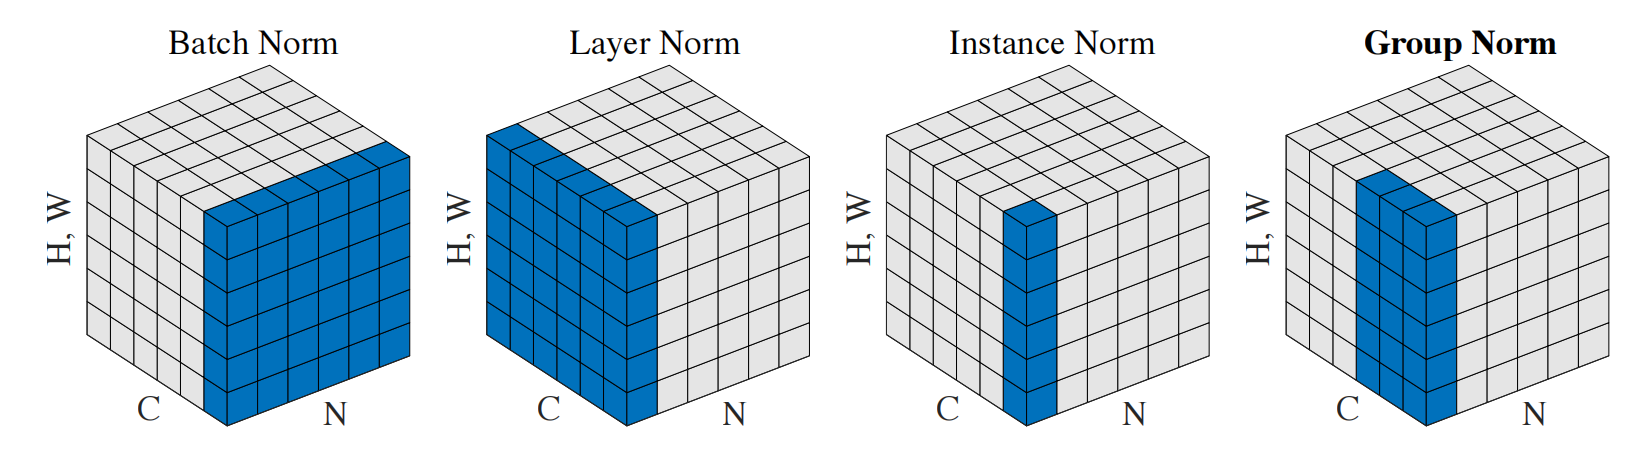
\includegraphics[width=0.8\textwidth]{figs/cnnnormlayer.png}
    \caption{Normalization methods for a CNN}
    {\footnotesize
    \textbf{BN}: pool over height and width in a batch, but match on the channel;
    \textbf{LN}: pool over channel, height and width, but match on the instance index in a batch;
    \textbf{IN}: pool over each instance in the batch and for each channel;
    \textbf{GN}: pool over all locations whose channel is in the same group.
    }
    \label{fig:cnnnormlayer}
\end{figure}